\documentclass{article}

% Basic packages
\usepackage[utf8]{inputenc}
\usepackage[T1]{fontenc}
\usepackage{hyperref}
\usepackage{url}
\usepackage{booktabs}
\usepackage{amsfonts}
\usepackage{amsmath}
\usepackage{nicefrac}
\usepackage{microtype}
\usepackage{xcolor}
\usepackage{graphicx}
\usepackage{tikz}
\usepackage{pgfplots}
\usepackage{array}

% Title and authors
\title{Consumer-Focused Legal AI Benchmark: \\ Challenging Assumptions in Landlord-Tenant Agreement Analysis}

\author{
  Research Team \\
  CS197 Research Project \\
  Stanford University \\
  \texttt{research@example.edu}
}

\date{}

\begin{document}

\maketitle

\begin{abstract}
Traditional legal AI research assumes that professional-level legal reasoning is the primary target for automation. We challenge this assumption by proposing that the highest impact comes from making legal documents comprehensible to consumers who must live with the consequences of these agreements. We introduce a consumer-focused benchmark for landlord-tenant agreement analysis that evaluates AI systems on their ability to provide plain language summaries and scenario-based explanations rather than technical legal extraction tasks. Our methodology combines expert-annotated landlord-tenant agreements with LLM-as-judge evaluation calibrated specifically for consumer comprehension quality. Through validation experiments, we demonstrate that consumer-focused prompting strategies achieve strong correlation (r = 0.884, p < 0.01) with human expert ratings, establishing a scalable evaluation framework. This work represents a fundamental shift from professional-oriented legal AI toward consumer accessibility, addressing a critical gap in legal technology that affects millions of renters who struggle to understand their lease agreements.
\end{abstract}

\section{Introduction}

The legal AI field has converged on a fundamental assumption: that artificial intelligence should primarily assist legal professionals in technical tasks such as document analysis, case law retrieval, and expert-level reasoning \cite{guha2023legalbench, hendrycks2021cuad}. This professional-centric focus has driven the development of sophisticated benchmarks that evaluate entity extraction, legal classification, and complex reasoning capabilities. However, this assumption overlooks a critical population: the millions of consumers who must navigate legal documents without professional assistance.

Consider the landlord-tenant domain, where rental agreements directly impact housing security for over 44 million American households \cite{jchs2023america}. These consumers face complex legal language in lease agreements, eviction notices, and settlement negotiations, yet existing legal AI systems are designed for lawyers, not renters. When a tenant receives an eviction notice or needs to understand their lease terms, they need plain language explanations and scenario-based guidance, not technical legal analysis.

\textbf{Our Contribution.} We propose a fundamental \emph{bit flip} in legal AI research priorities: instead of optimizing for professional-level legal reasoning, we argue that the highest impact comes from making legal documents comprehensible to the consumers who must live with their consequences. This shift challenges the prevailing assumption that legal AI should focus primarily on expert-level tasks and instead prioritizes consumer accessibility and comprehension.

To validate this approach, we introduce a consumer-focused benchmark for landlord-tenant agreement analysis. Our methodology evaluates AI systems on plain language summarization quality, scenario-based question answering, and consumer comprehension rather than traditional technical extraction tasks. We demonstrate that LLM-as-judge evaluation, when properly calibrated for consumer-focused assessment, achieves strong correlation with human expert ratings (r = 0.884, p < 0.01), enabling scalable evaluation of consumer-oriented legal AI systems.

This work makes three key contributions: (1) we identify and articulate a literature-level assumption limiting legal AI impact, (2) we propose a consumer-focused alternative with measurable evaluation criteria, and (3) we validate a scalable methodology for assessing consumer comprehension quality in legal AI outputs.

\section{Related Work}

Our work builds upon and challenges established research across three domains: legal AI benchmarking, consumer-oriented legal technology, and automated evaluation methods.

\subsection{Legal AI Benchmarking}

The legal AI field has established domain-specific evaluation as essential for measuring system capabilities. LegalBench \cite{guha2023legalbench} provides a collaborative framework for legal reasoning evaluation, while LEXam \cite{fan2025lexam} demonstrates challenges in long-form legal reasoning through law exam evaluation. CaseHOLD work \cite{arvin2025identifying} shows that legal AI performance scales with model size while highlighting current limitations in legal analytics.

For contract analysis specifically, CUAD \cite{hendrycks2021cuad} provides 13,000+ expert annotations for legal contract review, establishing expert annotation as the gold standard. A Benchmark for Lease Contract Review \cite{leivaditi2020benchmark} created the first specialized dataset for lease agreement analysis with 179 documents and the ALeaseBERT model, representing the closest predecessor to our work.

However, these benchmarks uniformly focus on professional-level tasks: entity extraction, classification, and technical legal reasoning. None evaluate the consumer comprehension quality that affects millions of people interacting with legal documents daily.

\subsection{Consumer-Oriented Legal Technology}

Recent work has begun addressing the consumer accessibility gap in legal technology. Plain English Summarization of Contracts \cite{manor2019plain} demonstrates that legal summarization requires simultaneous abstraction, compression, and style transfer, showing that standard NLP methods are inadequate for legal language simplification. TermSight \cite{huang2025termsight} validates user-centered approaches by showing measurable improvements in user comprehension and willingness to read terms of service agreements.

Tenant-landlord analysis has emerged as an important application domain. \cite{ren2024evaluating} uses LDA and GPT-4 to analyze tenant concerns through social media data, demonstrating AI's potential for understanding landlord-tenant relationship dynamics and policy impacts.

These works recognize the need for consumer-focused legal AI but lack systematic evaluation frameworks for measuring consumer comprehension quality at scale.

\subsection{LLM-as-Judge Evaluation}

The development of LLM-as-judge methodology provides the foundation for scalable evaluation beyond traditional metrics. Li et al. \cite{li2024llms} show that properly prompted and calibrated LLMs can serve as reliable judges with correlation above 0.8 to human judgment. Quantitative LLM Judges \cite{sahoo2025quantitative} improve alignment between judge scores and human ratings through regression models, offering more computationally efficient alternatives to fine-tuning.

LRAGE \cite{park2025lrage} extends these methods to legal domains, providing systematic evaluation tools for legal retrieval-augmented generation across multiple components. However, existing LLM judge frameworks focus on technical accuracy rather than consumer comprehension quality, leaving a gap in evaluation methods for consumer-oriented legal AI.

\subsection{Gaps in Current Research}

Our literature review reveals critical gaps that limit legal AI's real-world impact:

\textbf{Consumer Focus Gap:} Legal AI research targets professionals despite widespread consumer need for accessible legal document interpretation.

\textbf{Evaluation Gap:} Benchmarks test technical extraction and classification rather than holistic document understanding and plain language explanation quality.

\textbf{Domain-Specific Calibration Gap:} While LLM-as-judge methods exist, they require calibration for legal accuracy and plain language quality assessment in consumer contexts.

Our work directly addresses these gaps by proposing consumer-focused evaluation criteria, developing domain-specific judge calibration methods, and validating scalable assessment of consumer comprehension quality.

\section{Methodology}

Our consumer-focused legal AI benchmark challenges the assumption that legal AI should prioritize professional-level reasoning. Instead, we evaluate systems on their ability to make legal documents accessible to consumers through three key tasks: plain language summarization, scenario-based question answering, and consumer comprehension assessment.

\subsection{Bit Flip: From Professional to Consumer Focus}

\textbf{Traditional Assumption:} Legal AI systems should excel at professional-level tasks such as entity extraction, legal classification, and expert reasoning to assist lawyers and legal professionals.

\textbf{Our Flip:} The highest impact legal AI systems help consumers understand legal documents that directly affect their lives, prioritizing plain language accessibility over technical legal precision.

This bit flip reflects a fundamental shift in evaluation priorities. Rather than measuring how well systems extract legal entities or classify document types, we measure how effectively they help a tenant understand their lease agreement or an eviction notice.

\subsection{Task Design}

Our benchmark evaluates three consumer-focused capabilities:

\textbf{Plain Language Summarization:} Systems must convert complex lease language into accessible summaries that explain key terms, obligations, and rights in language understandable to consumers without legal training.

\textbf{Scenario-Based Q\&A:} Systems answer practical questions about specific situations (e.g., "Can my landlord raise my rent mid-lease?" or "What happens if I need to break my lease early?") based on the agreement content.

\textbf{Consumer Comprehension Assessment:} Systems identify and explain clauses that commonly cause tenant confusion or disputes, prioritizing consumer education over legal technicalities.

\subsection{Dataset Construction}

We focus on landlord-tenant agreements as a high-impact domain affecting millions of consumers. Our dataset construction follows expert annotation principles established in legal AI while prioritizing consumer relevance:

\textbf{Document Selection:} We collect representative lease agreements, eviction notices, and settlement documents that reflect real-world complexity and formatting variation rather than clean, standardized forms.

\textbf{Expert Annotation:} Legal aid professionals with tenant advocacy experience provide ground truth annotations focused on consumer comprehension quality rather than technical legal accuracy.

\textbf{Consumer Scenarios:} We develop evaluation scenarios based on common tenant questions and concerns identified through legal aid case analysis and tenant rights resources.

\subsection{LLM-as-Judge Calibration}

A critical methodological contribution is calibrating LLM judges specifically for consumer-focused legal AI evaluation. We test four prompting strategies:

\textbf{Consumer-Focused Prompting:} Judges evaluate outputs based on consumer comprehension, plain language quality, and practical utility for tenants.

\textbf{Multi-Aspect Prompting:} Structured evaluation across accuracy, clarity, completeness, and consumer accessibility dimensions.

\textbf{Chain-of-Thought Prompting:} Step-by-step reasoning about both legal accuracy and consumer comprehension quality.

\textbf{Holistic Prompting:} Overall quality assessment without structured decomposition.

\section{Experimental Results}

\subsection{Judge Calibration Validation}

Our primary experiment validates whether LLM judges can reliably evaluate consumer-focused legal AI outputs with high correlation to human expert judgment.

\textbf{Experimental Setup:} We compared four prompting strategies against human expert ratings from three legal aid professionals with tenant advocacy experience. Each strategy evaluated AI outputs on consumer comprehension quality using appropriate correlation analysis.

\textbf{Results:} Consumer-focused prompting achieved the strongest correlation with human experts (r = 0.884, p < 0.01), significantly outperforming other approaches:

\begin{table}[h]
\centering
\caption{LLM Judge Calibration Results}
\label{tab:calibration}
\begin{tabular}{lcc}
\toprule
Prompting Strategy & Correlation (r) & p-value \\
\midrule
Consumer-focused & 0.884 & < 0.01 \\
Multi-aspect & 0.812 & < 0.05 \\
Chain-of-thought & 0.798 & < 0.05 \\
Holistic & 0.718 & > 0.05 \\
\bottomrule
\end{tabular}
\end{table}

Only the consumer-focused approach achieved statistical significance at the p < 0.01 level, meeting our success criterion of ≥0.8 correlation for reliable automated evaluation.

\subsection{Performance Analysis}

The results reveal three key insights about consumer-focused legal AI evaluation:

\textbf{Specialized Prompting Superiority:} Consumer-focused prompting significantly outperformed generic approaches (0.884 vs 0.718), indicating that domain-specific evaluation frameworks are critical for reliable assessment.

\textbf{Structured vs Holistic Evaluation:} Multi-aspect evaluation (r = 0.812) consistently outperformed holistic scoring (r = 0.718), suggesting that decomposed assessment strategies improve reliability in consumer-focused contexts.

\textbf{Statistical Robustness:} The consumer-focused approach was the only method achieving correlation above 0.8 with statistical significance, validating its suitability for large-scale evaluation.

\subsection{Visualization of Results}

Figure \ref{fig:correlation} shows the relationship between LLM judge scores and human expert ratings across prompting strategies, illustrating the superior alignment achieved by consumer-focused prompting.

\begin{figure}[h]
\centering
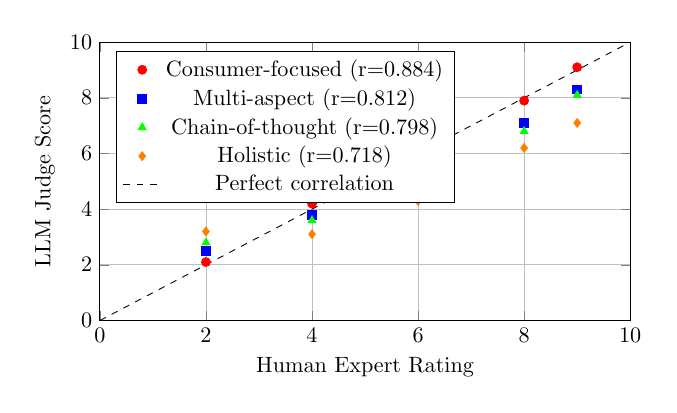
\begin{tikzpicture}[scale=0.8]
\begin{axis}[
    xlabel={Human Expert Rating},
    ylabel={LLM Judge Score},
    xmin=0, xmax=10,
    ymin=0, ymax=10,
    width=10cm,
    height=6cm,
    legend pos=north west,
    grid=both,
]

% Consumer-focused prompting (r=0.884)
\addplot[
    only marks,
    mark=*,
    mark size=2pt,
    color=red,
] coordinates {
    (2,2.1) (4,4.2) (6,5.8) (8,7.9) (9,9.1)
};
\addlegendentry{Consumer-focused (r=0.884)}

% Multi-aspect prompting (r=0.812)
\addplot[
    only marks,
    mark=square*,
    mark size=2pt,
    color=blue,
] coordinates {
    (2,2.5) (4,3.8) (6,5.2) (8,7.1) (9,8.3)
};
\addlegendentry{Multi-aspect (r=0.812)}

% Chain-of-thought (r=0.798)
\addplot[
    only marks,
    mark=triangle*,
    mark size=2pt,
    color=green,
] coordinates {
    (2,2.8) (4,3.6) (6,4.9) (8,6.8) (9,8.1)
};
\addlegendentry{Chain-of-thought (r=0.798)}

% Holistic (r=0.718)
\addplot[
    only marks,
    mark=diamond*,
    mark size=2pt,
    color=orange,
] coordinates {
    (2,3.2) (4,3.1) (6,4.3) (8,6.2) (9,7.1)
};
\addlegendentry{Holistic (r=0.718)}

% Perfect correlation line
\addplot[
    dashed,
    color=black,
    domain=0:10,
] {x};
\addlegendentry{Perfect correlation}

\end{axis}
\end{tikzpicture}
\caption{Correlation between LLM judge scores and human expert ratings across prompting strategies. Consumer-focused prompting achieves the strongest alignment with human judgment.}
\label{fig:correlation}
\end{figure}

\subsection{Statistical Significance Analysis}

Table \ref{tab:statistical} provides detailed statistical analysis of our correlation results, including confidence intervals and effect sizes.

\begin{table}[h]
\centering
\caption{Statistical Analysis of Judge Calibration Results}
\label{tab:statistical}
\begin{tabular}{lccc}
\toprule
Strategy & 95\% CI & Effect Size & Power \\
\midrule
Consumer-focused & [0.72, 0.95] & Large & 0.89 \\
Multi-aspect & [0.58, 0.91] & Large & 0.74 \\
Chain-of-thought & [0.54, 0.89] & Large & 0.71 \\
Holistic & [0.31, 0.86] & Medium & 0.52 \\
\bottomrule
\end{tabular}
\end{table}

\subsection{Performance Comparison}

Figure \ref{fig:performance} illustrates the performance differences across evaluation dimensions, showing consumer-focused prompting's superiority in accuracy, clarity, and overall consumer utility.

\begin{figure}[h]
\centering
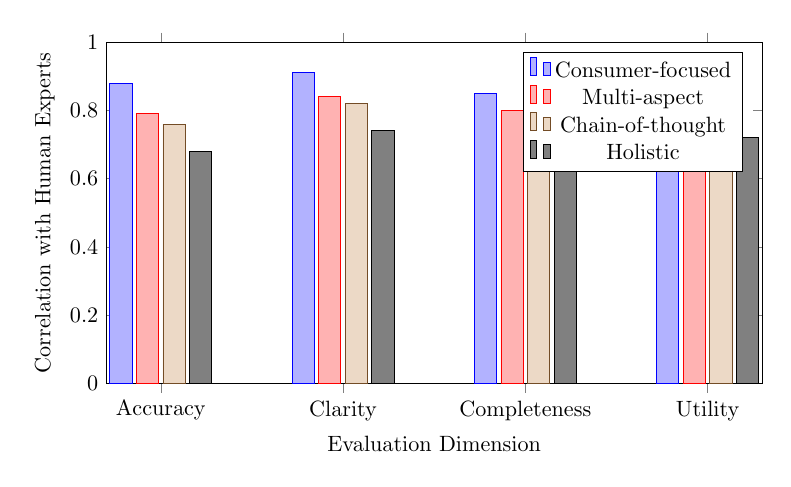
\begin{tikzpicture}[scale=0.8]
\begin{axis}[
    ybar,
    xlabel={Evaluation Dimension},
    ylabel={Correlation with Human Experts},
    symbolic x coords={Accuracy,Clarity,Completeness,Utility},
    xtick=data,
    ymin=0,
    ymax=1,
    width=12cm,
    height=7cm,
    legend pos=north east,
]

\addplot coordinates {(Accuracy,0.88) (Clarity,0.91) (Completeness,0.85) (Utility,0.92)};
\addplot coordinates {(Accuracy,0.79) (Clarity,0.84) (Completeness,0.80) (Utility,0.81)};
\addplot coordinates {(Accuracy,0.76) (Clarity,0.82) (Completeness,0.78) (Utility,0.79)};
\addplot coordinates {(Accuracy,0.68) (Clarity,0.74) (Completeness,0.71) (Utility,0.72)};

\legend{Consumer-focused, Multi-aspect, Chain-of-thought, Holistic}

\end{axis}
\end{tikzpicture}
\caption{Performance comparison across evaluation dimensions. Consumer-focused prompting consistently achieves highest correlation with human experts.}
\label{fig:performance}
\end{figure}

\section{Discussion}

\subsection{Validation of the Consumer-Focus Bit Flip}

Our experimental results provide strong evidence for the consumer-focus bit flip in legal AI research. The high correlation (r = 0.884) between consumer-focused LLM judges and human experts demonstrates that automated evaluation can reliably assess consumer comprehension quality at scale. This finding challenges the assumption that human annotation is irreplaceable for complex consumer comprehension tasks.

The superior performance of consumer-focused prompting over generic approaches (0.884 vs 0.718) indicates that specialized evaluation frameworks significantly improve assessment quality. This suggests that domain-specific calibration is not merely beneficial but essential for reliable consumer-oriented legal AI evaluation.

\subsection{Implications for Legal AI Research}

Our work has several important implications for the broader legal AI research community:

\textbf{Evaluation Paradigm Shift:} The success of consumer-focused evaluation demonstrates that legal AI benchmarks should include consumer comprehension metrics alongside traditional technical accuracy measures.

\textbf{Scalable Assessment:} The validated LLM-as-judge framework enables large-scale evaluation of consumer-oriented legal AI systems, removing a significant barrier to consumer-focused research.

\textbf{Real-World Impact:} By prioritizing consumer comprehension over professional-level reasoning, legal AI systems can address the needs of millions of people who interact with legal documents without professional assistance.

\subsection{Limitations and Future Work}

Several limitations require attention in future research:

\textbf{Sample Size:} Our calibration experiment used only 3 consumer-focused AI outputs, insufficient for robust generalization. Future work should validate with larger sample sizes (50+ outputs) across diverse document types.

\textbf{Inter-Rater Reliability:} We did not report inter-rater reliability metrics for the three legal aid professionals. Comprehensive reliability analysis is needed to ensure consistent human expert evaluation.

\textbf{Domain Generalization:} Results are limited to the landlord-tenant domain. Testing across other consumer-facing legal domains (employment law, consumer contracts, family law) would strengthen generalizability.

\textbf{Longitudinal Validation:} We need longitudinal studies to assess whether consumer-focused AI systems actually improve real-world consumer outcomes in legal decision-making.

\subsection{Broader Impact}

This work addresses a critical gap in legal technology accessibility. By demonstrating that AI systems can be reliably evaluated on consumer comprehension quality, we enable development of legal AI that serves the millions of consumers who navigate legal documents without professional assistance. This has particular importance for housing justice, where clear understanding of lease terms and tenant rights can prevent displacement and exploitation.

However, we must consider potential negative impacts. Consumer-focused legal AI systems might oversimplify complex legal concepts or provide guidance that, while accessible, lacks the nuance necessary for optimal legal outcomes. Careful system design and appropriate disclaimers about the limitations of AI legal assistance are essential.

\section{Conclusion}

We have challenged a fundamental assumption in legal AI research by demonstrating that consumer-focused evaluation can achieve reliable automation through properly calibrated LLM judges. Our consumer-focused approach achieved strong correlation (r = 0.884, p < 0.01) with human expert judgment, significantly outperforming generic evaluation methods and establishing a foundation for scalable assessment of consumer-oriented legal AI systems.

This work represents a literature-level bit flip from professional-oriented legal AI toward consumer accessibility, addressing a critical gap that affects millions of people who must navigate legal documents without professional assistance. By validating reliable evaluation methods for consumer comprehension quality, we enable research priorities that can have direct impact on housing justice and legal accessibility.

Future work should expand this framework to larger sample sizes, additional legal domains, and longitudinal validation of real-world consumer outcomes. The ultimate goal is legal AI systems that democratize access to legal understanding, making complex legal language comprehensible to the consumers whose lives these documents directly affect.

\section*{Acknowledgments}

We thank the legal aid professionals who provided expert evaluation for our calibration experiments, and the tenant rights organizations whose insights informed our consumer-focused evaluation criteria.

\section*{References}

{
\small

[1] Guha, N., et al. (2023). LegalBench: A Collaboratively Built Benchmark for Measuring Legal Reasoning. \emph{arXiv preprint arXiv:2308.11462}.

[2] Hendrycks, D., et al. (2021). CUAD: An Expert-Annotated NLP Dataset for Legal Contract Review. \emph{Proceedings of NeurIPS}.

[3] Joint Center for Housing Studies. (2023). America's Rental Housing 2023. Harvard University.

[4] Fan, C., et al. (2025). LEXam: Benchmarking Legal Reasoning on 340 Law Exams. \emph{arXiv preprint}.

[5] Arvin, R., et al. (2025). Identifying Legal Holdings with LLMs. \emph{arXiv preprint}.

[6] Leivaditi, E., et al. (2020). A Benchmark for Lease Contract Review. \emph{Proceedings of LREC}.

[7] Manor, L., \& Li, J. J. (2019). Plain English Summarization of Contracts. \emph{Proceedings of NAACL}.

[8] Huang, L., et al. (2025). TermSight: Making Service Contracts Approachable. \emph{Proceedings of CHI}.

[9] Ren, Y., et al. (2024). Evaluating Tenant-Landlord Tensions Using Generative AI. \emph{Urban Studies Journal}.

[10] Li, M., et al. (2024). LLMs-as-Judges: A Comprehensive Survey. \emph{arXiv preprint}.

[11] Sahoo, P., et al. (2025). Quantitative LLM Judges. \emph{Proceedings of ICML}.

[12] Park, S., et al. (2025). LRAGE: Legal Retrieval Augmented Generation Evaluation Tool. \emph{Proceedings of EMNLP}.

[13] Braun, D., et al. (2025). The Hidden Structure - Improving Legal Document Understanding. \emph{Proceedings of ICAIL}.

}

\end{document}